Phase-Sensitive Detectors (PSD) present an alternative to LIA. PSD uses square signals and an inverter to switch between the original and inverted version of the signal of interest at the frequency of the square reference signal \cite{horowitz1989art}. This switching creates a signal with frequency components at DC and at two times the reference signal. After passing through a low-pass filter, only the DC component proportional to the real and imaginary current of the SUT’s impedance remains. The behavior and implementation of a PSD is shown in figure \autoref{fig:PSD_circuit}. The main advantage of PSDs is that they replace the complex hardware associated with conventional sinewave spectroscopy with much simpler clock-based circuitry \cite{Subhan2019}. For instance, the DAC, wave generator, and linear mixer can all be replaced by a simple clock generator and controlled switches. This leads to a decrease of the system’s power-consumption, which is primordial in portable application \cite{Subhan2019}. \par
\begin{figure}[h]
    \centering
    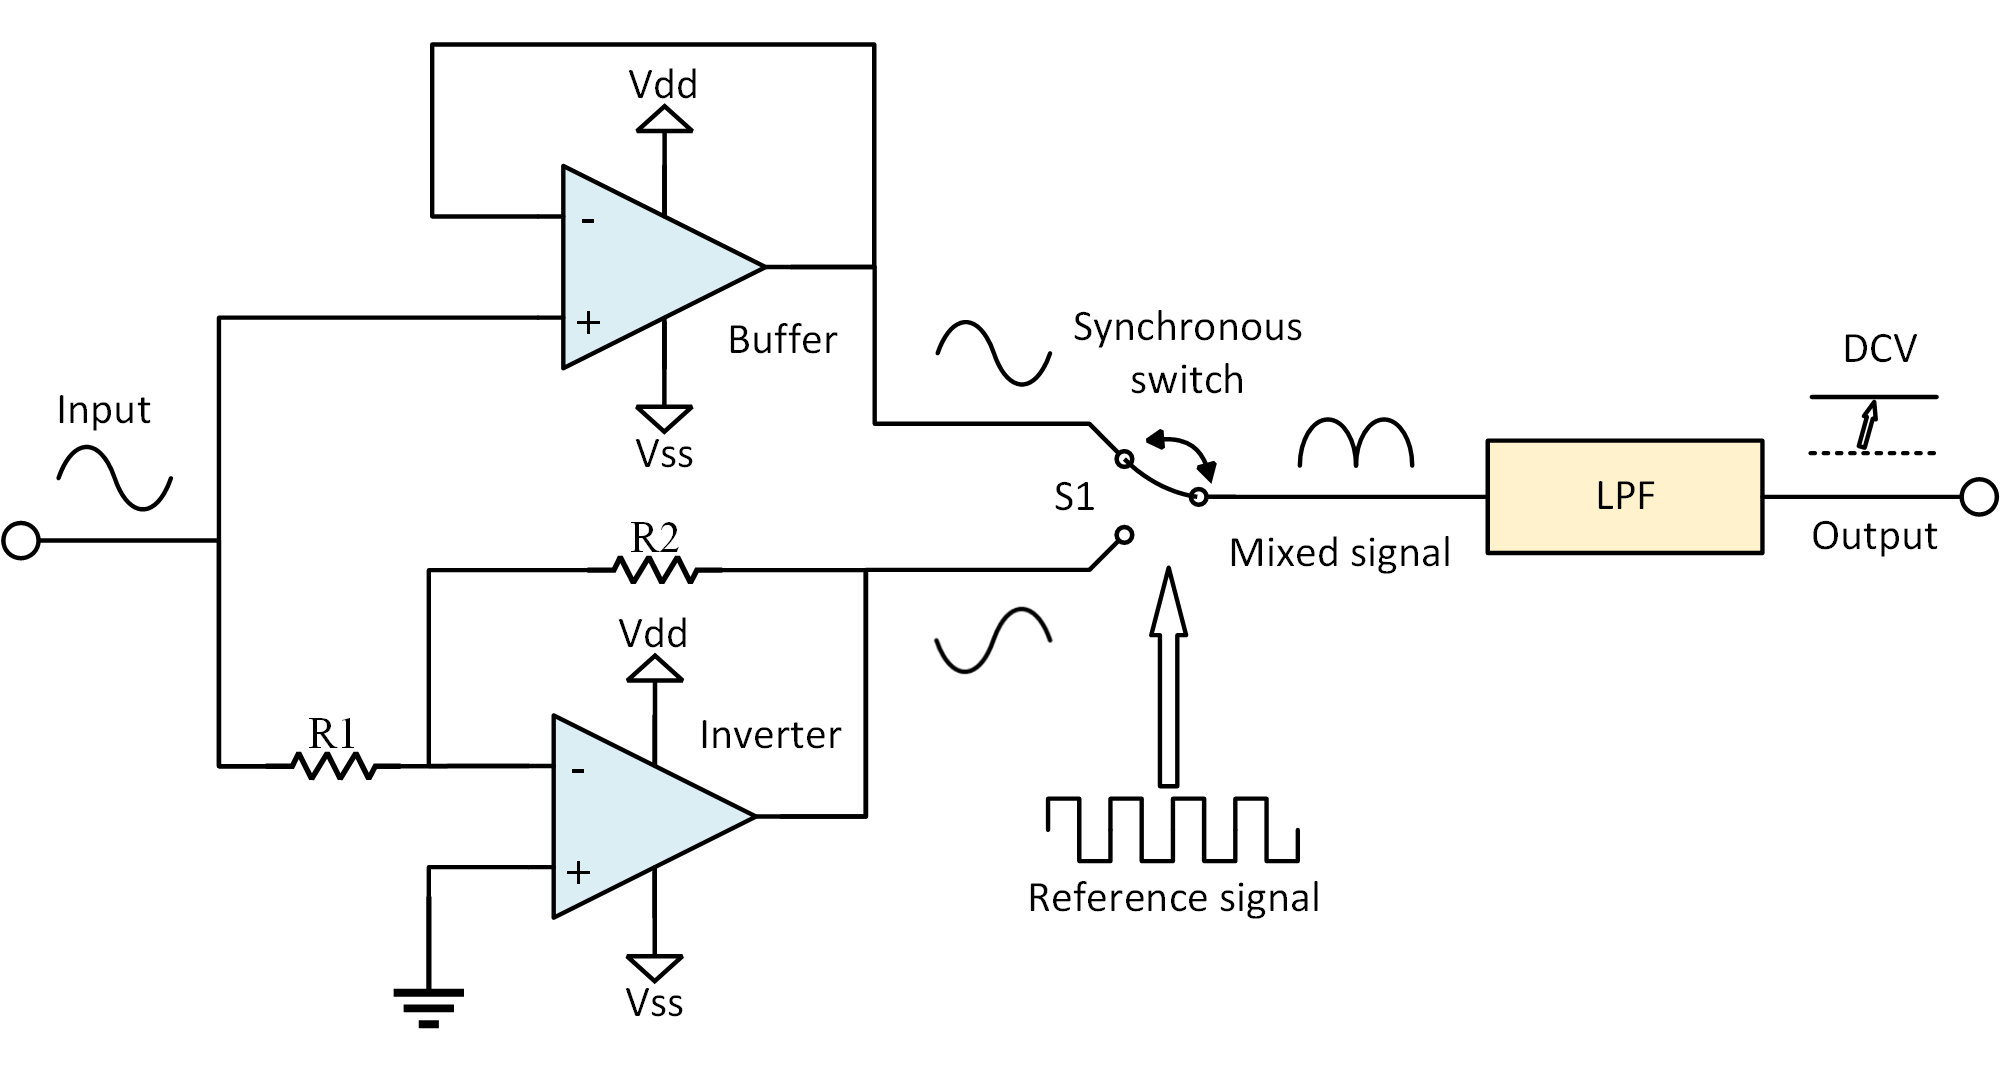
\includegraphics[width=1\textwidth]{PSD_circuit}
    \caption{Behavior and implementation of a PSD circuit.}
    \label{fig:PSD_circuit}
\end{figure}
PSD are, however, less precise compared to LIAs or other systems based on sinewaves. As will be described in \autoref{sec:ImpedancePrinciples}, using square waves introduce a systematic error in the amplitude measurement, which can be mostly corrected in post-processing if multiple frequency points are sampled. This error introduces errors of less than 2\%. Another consideration is the introduction of harmonics in the system, which raises the noise floor of the circuit \cite{Subhan2019}. 